\chapter{Selección de equipamiento, despliegue y diseño de la red}
\label{cap:equipamiento}

\section{Comparación entre equipos}	
Antes de proceder a comparar los equipos introducidos anteriormente, debemos primero explicar el protocolo de pruebas que se ha elaborado con la colaboración de los compañeros involucrados pertenecientes a la PUCP. Dicho protocolo nos servirá para valorar y evaluar las prestaciones de cada uno de los equipos de forma individual y establecer una comparativa, con el fin de obtener una solución lo más viable y factible posible en lo que al marco del proyecto se refiere. \\

 Primeramente se van a establecer, con ayuda de RadioMobile, los requisitos mínimos de los equipos que pueden ser elegibles para su uso en los enlaces de la red que se va a desplegar; a partir de esos requisitos, se ha diseñado un protocolo de pruebas en colaboración con la PUCP que comporta revisión de las especificaciones y pruebas de campo con los equipos. Las pruebas de campo conllevarán la configuración de un enlace punto a punto en las instalaciones disponibles para dicho efecto de la PUCP. Una vez configurado el enlace, se realizarán pruebas de conectividad utilizando programas para inyectar tráfico y se examinarán los valores obtenidos. De forma simultánea, se registrarán los valores energéticos proporcionados por los equipos durante las pruebas para valorar su eficiencia energética.\\
 
 Las pruebas realizadas por la PUCP han sido llevadas a cabo en diferentes emplazamientos, ubicados en Iquitos-Mazán para el caso de los equipos Net Metal 5 y RM-MAX, y por otro lado para los equipos Ubiquiti en los emplazamientos encontrados en Pachatutec (Ventanilla) y San Miguel. Aunque a simple vista parezca que la ubicación de los emplazamientos seleccionados es muy dispar, la infraestructura existente y sus perfiles geográficos son muy parejos, por lo tanto nos sirve como escenario para realizar nuestro análisis. De igual forma, este estudio se ha tenido que realizar de forma interrumpida, es decir primero una pareja de equipos y después la otra, debido a las disponibilidad de los emplazamientos y equipos.\\
 
 La configuración de ambos escenarios sigue un esquema similar al mostrado en la Figura \ref{pruebasPUCP}, en este caso particular se hace referencia al enlace existente entre Mázan y el hospital regional de Loreto y las características utilizadas para el desarrollo de pruebas en dicho emplazamiento. No obstante esta arquitectura es la utilizada a lo largo de todos los emplazamientos que conforman la red del Napo, dicha arquitectura está compuesta por torres metálicas y equipos portátiles en los cuales se realizarán las mediciones de tráfico y se medirá el rendimiento de los equipos.
 
 \begin{figure}[H]
			\centering
			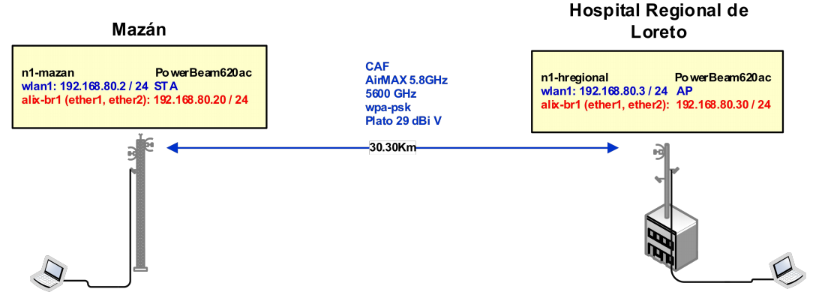
\includegraphics[width=0.7\textwidth]{img/enlace.PNG}
			\caption{Escenario de pruebas propuesto por PUCP.}
			\label{pruebasPUCP}
\end{figure}

Antes de comenzar a detallar los resultados obtenidos en cada una de las pruebas realizadas, debemos aclarar los criterios y exigencias mínimas a las que los equipos han sido sometidas. Dichos requerimientos se describen a continuación:

\begin{itemize}
    \item La gestionabilidad de los equipos se realizará mediante el protocolo SNMP, por tanto debemos disponer de la MIB del fabricante y programa para gestionar los equipos con el objetivo de monitorizar y configurar las pruebas a realizar.
    \item Diseñar un perfil virtual obtenido a través de RadioMobile configurado con las características de los equipos.
    \item La calidad del radio enlace establecido ha de tener un nivel de señal satisfactorio. Considerando satisfactorio una potencia de señal recibida que quede al menos 15 dB por encima de la sensibilidad del modo de transmisión más robusto que sea utilizable.
\end{itemize}

Por último, y en adición a todo lo comentado anteriormente, se crearán unos cuadros de emparejamiento con los equipos y sus principales características junto a los datos obtenidos en las pruebas para así extraer una conclusión sobre qué equipo es el propuesto como solución en este proyecto.

\subsection{Comparación NetMetal 5 - RM-MAX}
 Este primer análisis se ha llevado a cabo en los emplazamientos de San Miguel y Ventanilla los cuales están separados por una distancia de 29 Km y disponen de torres con antenas cuya ganancia es de 34 dBi en la banda de 5 GHz. Para llevar a cabo las pruebas de tráfico  y eficiencia se han tenido en cuenta los resultado obtenidos en los perfiles obtenidos con la simulación, correspondientes a las imágenes \ref{mikro_sanmiguel} y \ref{mikro_rmmax}; y los datos recopilados en la Tabla \ref{table:parámetrosEquipos} que identifican los principales parámetros de los equipos.\\
 
  \begin{figure}[H]
			\centering
			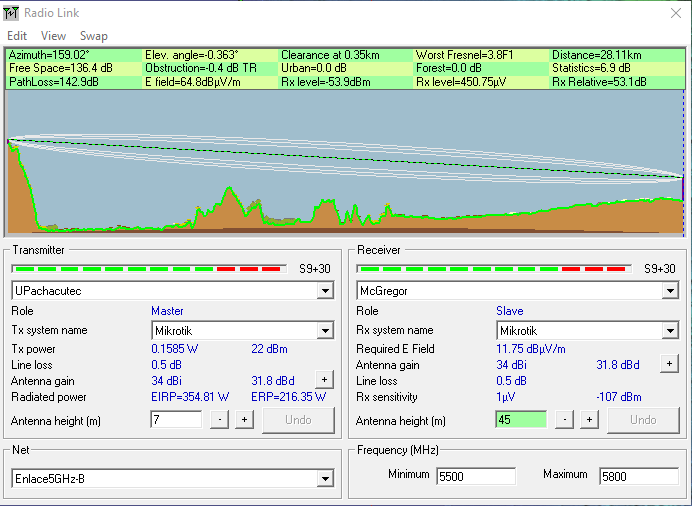
\includegraphics[width=0.6\textwidth]{img/Mikrotik_pruebas.png}
			\caption{Simulación realizada con la configuración de equipos NetMetal 5 entre las estaciones de San Miguel y Ventanilla}
			\label{mikro_sanmiguel}
\end{figure}
 \begin{figure}[H]
			\centering
			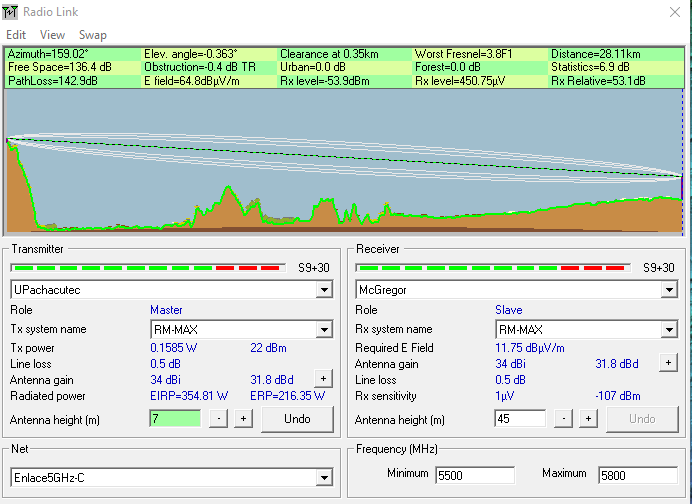
\includegraphics[width=0.6\textwidth]{img/rmmax_pruebas.png}
			\caption{Simulación realizada con la configuración de equipos RM-MAX entre las estaciones de San Miguel y Ventanilla}
			\label{mikro_rmmax}
\end{figure}
 Una vez identificado los primeros valores de viabilidad del enlace, el siguiente paso es realizar pruebas teniendo en cuenta la variación de ancho del canal y la modulación utilizada. En este caso se utilizó la frecuencia de 5745 MHz como frecuencia operacional, y 20 - 40 MHz como valores de ancho de banda. Por último, se determinó fijar el valor de la modulación de transmisión en una MCS11, correspondiente a una constelación 16QAM, por considerarse la más robusta elegible en función de la capacidad binaria que va a brindar. Los resultados obtenidos se muestran en la Tabla \ref{table:pruebasEquipos}; dicha tabla recoge los promedios obtenidos en cuanto al porcentaje de paquetes pérdidos, retardo y \textit{throughput}.\\ 
Una vez examinado los datos obtenidos en las pruebas realizadas vemos como los equipos Mikrotik ofrecen mejor rendimiento y prestaciones tanto para el ancho de canal de 20 MHz como para el de 40 MHz respecto al equipo RM-MAX. \\

Mientras que los equipos RM-MAX tienen un \textit{throughput} de 1,42 Mbps, 46\% de paquetes pérdidos y 223 ms de retardo todo ello para 20 MHz, frente a los 10 Mbps, 12\% y 11 ms que ofrecen los equipos Net Metal 5. Para el ancho de banda de 40 MHz los resultados siguen siendo iguales, para los valores de 45 Kbps, 63\% y 168 ms que ofrecidos por los equipos RM-MAX, los equipos NetMetal 5 ofrecen valores de 24,32 Mbps, 0,46\% y 10 ms.\\

En cuanto al consumo energético, los equipos NetMetal 5 consumen 8,35 W mientras que los equipos RM-MAX llevan su consumo hasta 14,29 W de potencia.\\

A la vista de los resultados, los equipos NetMetal 5 son los equipos elegidos como solución frente a los RM-MAX. 

\subsection{Comparación PowerBeam AC - AirFiber }
Para este segundo análisis los emplazamientos escogidos fueron los ubicados en Mazán e Iquitos entre los cuales existe una distancia de aproximadamente 31 Km. Para llevar a cabo estas pruebas y perfiles greográficos con RadioMobile, se parametrizaron las configuraciones de los equipos acorde a la Tabla \ref{table:parámetrosEquiposUbiquiti} y teniendo en cuenta las restricciones existentes en cuanto a la potencia isotrópica radiada equivalente (PIRE), la cual se establece en 49 dBm para el primer rango de frecuencias y en 54 dBm para el cuarto rango de frecuencias.\\

Por un lado, para conocer la viabilidad del enlace y establecer un mínimo de potencia que garantice la estabilidad del mismo, se han utilizado los perfiles obtenidos en la simulación, dichos perfiles están ubicados a contiuación en la Figura \ref{simulacionUbiquiti}. Una vez analizado los perfiles se observa como para el primer rango de frecuencias, existe un limitación de potencia transmitida a nivel legislativo, por tanto nuestra simulación no puede exceder dichos valores. El resultado de la simulación establece que el mínimo de potencia de señal recibidad es de 21,9 dBm con los equipos AirFiber y 23,2 dBm para los equipos PowerBeam.

\begin{figure}[H]
\centering
\subfigure[Simulación con PowerBeam AC]{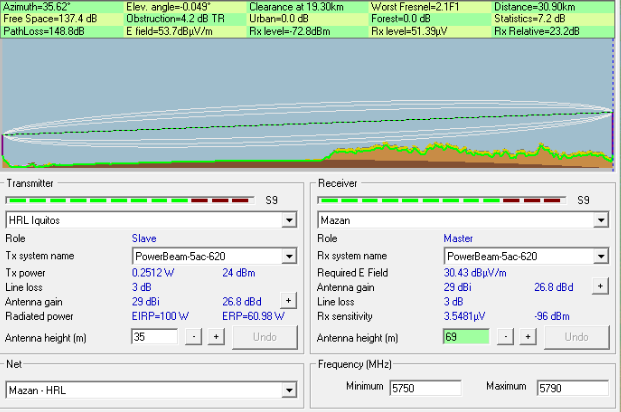
\includegraphics[width=70mm]{img/PowerBeamAC.PNG}}\hspace{2mm}
\subfigure[Simulación con AirFiber con 24 dBm de potencia de transmisión ]{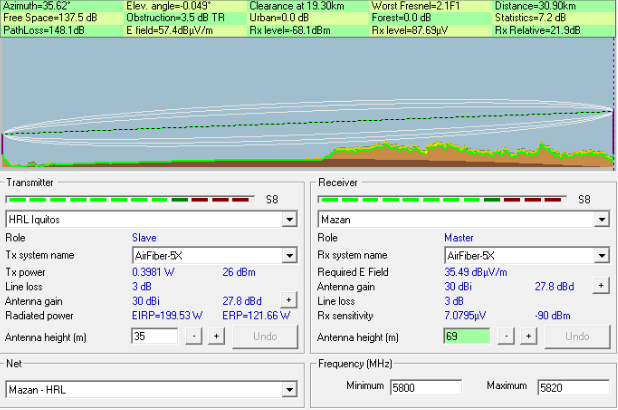
\includegraphics[width=70mm]{img/AirFiber5x.PNG}}\vspace{2mm}
\subfigure[Simulación con AirFiber con 22 dBm de potencia de transmisión]{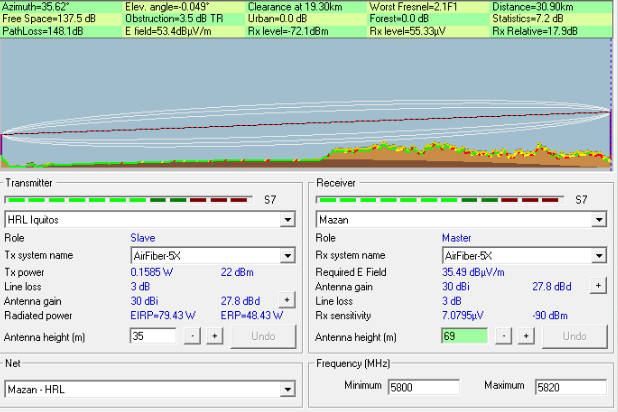
\includegraphics[width=70mm]{img/AirFiber5x_22dBm.PNG}}\hspace{2mm}
\subfigure[Simulación con AirFiber con 9 dBm de potencia de transmisión]{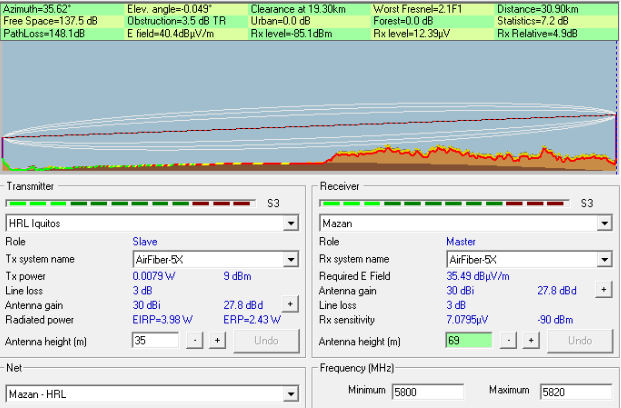
\includegraphics[width=71mm]{img/AirFiber5x_9dBm.PNG}}\vspace{2mm}
\caption{Simulación de los equipos Ubiquiti en el escenario Mazán-Iquitos} \label{simulacionUbiquiti}
\end{figure}

A parte de las pruebas con el escenario  simulado, se llevaron a cabo pruebas a nivel de campo con los equipos con el objetivo de conocer el rendimiento de cada uno de ellos; dichos resultados se adjuntan en la Tabla \ref{table:pruebasEquiposUbiquiti}. Una vez recopilados todos los datos y analizados, se extraen las siguientes conclusiones:

\begin{itemize}
    \item Bajo las condiciones de este escenario, los equipos PowerBeam son más estables utilizando un canal de 20 MHz, obteniendo una tasa de transferencia promedio de 40 Mbps. Por otra parte,los equipos AirFiber están alcanzando promedios de 37 Mbps utilizando un canal de 40 MHz y 78 Mbps utilizando un canal 50 MHz, aunque en ambos casos el enlace presenta inestabilidad.
    \item El retardo ofrecido por los equipos AirFiber es mucho mejor que el de los equipos PowerBeam.
    \item En la estación de Iquitos existe una abundante interferencia electromagnética lo que implica configurar de forma fija la modulación máxima, en Mazán se alcanza la modulación 64QAM mientras que en Iquitos se llega a la modulación 16QAM. En las mejores condiciones usando Powerbeam con un ancho de canal 20 MHz y retardos considerables conseguimos transmitir con la modulación de 64QAM; sin embargo, en el caso de Airfiber se consigue transmitir con una modulación de 16QAM con un ancho de canal de 40 MHz y bajo retardo.
\end{itemize}

Una vez comtemplando los diferentes equipos y habiendo realizado pruebas en el escenario destinado para ello y en entornos simulados, los equipos propuestos como solución a usar en el marco de este proyecto son los NetMetal 5. Gracias a su mejor rendimiento en el conjunto global de la evaluación, teniendo en cuenta su eficiencia energética, versatilidad a la hora de establecer configuraciones y manejo de la herramienta de configuración, desempeño durante las pruebas de ancho de badna y tráfico.

\section{Configuración y diseño de la red}
Antes de realizar el montaje del escenario y realización de pruebas en laboratorio, debemos realizar un diseño y estudio sobre la red. Dicho análisis nos permitirá conocer de forma más detallada los diferentes factores que pueden comprometer la viabilidad de los diferentes enlaces que componen la red, y así ajustar la configuración de los equipos a dichos factores para garantizar el objetivo y requisitos predefinidos en el proyecto.\\

Tras la conlcusión de la parte correspondiente al estudio y diseño de la red, realizaremos nuestras simulaciones a nivel de laboratorio. El objetivo de esto será establecer una comparación con los resultados obtenidos en la fase de estudio; para ello dispondremos de los equipos NetMetal 5 y ordenadores con sistema operativo GNU/Linux, ya que este sistema operativo da facilidades añadidas a la hora de instalar y manejar los programas necesarios para la realización de pruebas. Las pruebas llevadas a cabo determinarán el rendimiento que ofrecen los equipos NetMetal 5 en lo que a conectividad y parámetros de calidad se refiere.

\subsection{Estudio previo} 
	En esta sección procederemos a realizar un estudio teórico cuantitativo del \textit{throughput} que se puede esperar en cada uno de los radioenlaces que forman la red del Napo. Para ello utilizaremos los valores empíricos obtenidos en el artículo \cite{simo2014assessing} recogidos en la Tabla \ref{table:pruebasNV2campo}, obtenidos a través de la realización de pruebas de campo con el protocolo NV2 y un ancho de banda de 20 MHz.\\
	
	Por una parte, los valores presentes en dicha tabla corresponden a medidas de capacidad en radioenlace para una distancia de 0 Km (medidas en laboratorio) y una distancia de 30 Km, las medidas fueron llevadas a cabo desde la modulación MCS0 hasta MCS15 para la mayoría de casos, salvo en las mediciones de 30 Km, qué para valores superiores a MCS11 no se pudieron realizar pruebas empirícas. No obstante, sólo nos apoyaremos y tomaremos como referencia los valores comprendidos entre la modulación MCS8 y MCS11 ya que son las modulaciones destinadas para el uso de MIMO. \\
	Por otra parte, dichas medidas corresponden a la utilización de 20 Mhz como ancho de banda, para poder establecer una relación con el ancho de banda utilizado en el proyecto se procederá a duplicar los valores obtenidos a 20 Mhz. Obteniendo así un aproximación de los valores teóricos que deberían ser obtenidos de forma empiríca para un ancho de banda de 40 Mhz; una vez concluida la parte teórica se contrastarán dichos valores con los obtenidos en laboratorio y se procederá a realizar un análisis más exhaustivo.\\
	
	Para poder llevar a cabo el estudio teórico, se han recogido los valores antes mencionados y se han organizado en pares de coordenadas obteniendo un conjunto de datos que establecen una relación entre: la distancia, el \textit{throughput}, y el valor de la modulación MCS utilizado. Una vez acondicionados los datos, se ha proyectado una recta lineal entre los puntos pertenecientes a cada MCS respecto a las coordenadas base de 0 Km y 30 Km, con el objetivo de obtener una recta que pase por todos los puntos de interés de nuestra red, tal y como muestra la Figura \ref{rectaspendiente}, permitiendo establecer así una aproximación teórica de la capacidad del enlace en función de la distancia.\\
	
	De forma paralela, en base a la obtención de las rectas respecto a cada MCS hemos podido realizar una estimación de la capacidad teórica que debería de existir para cada radioenlace; dicha estimación se muestra en la Figura \ref{valoresmbps}. Para llevar a cabo todo el estudio teórico y todo el desarrollo comentado anteriormente, se ha utilizado el script \ref{lst:script}, que está desarrollado en el lenguaje de programación Python, ya que permite la integración de módulos y librerías de análisis matemático de forma sencilla.
	
	\begin{figure}[H]
		\centering
		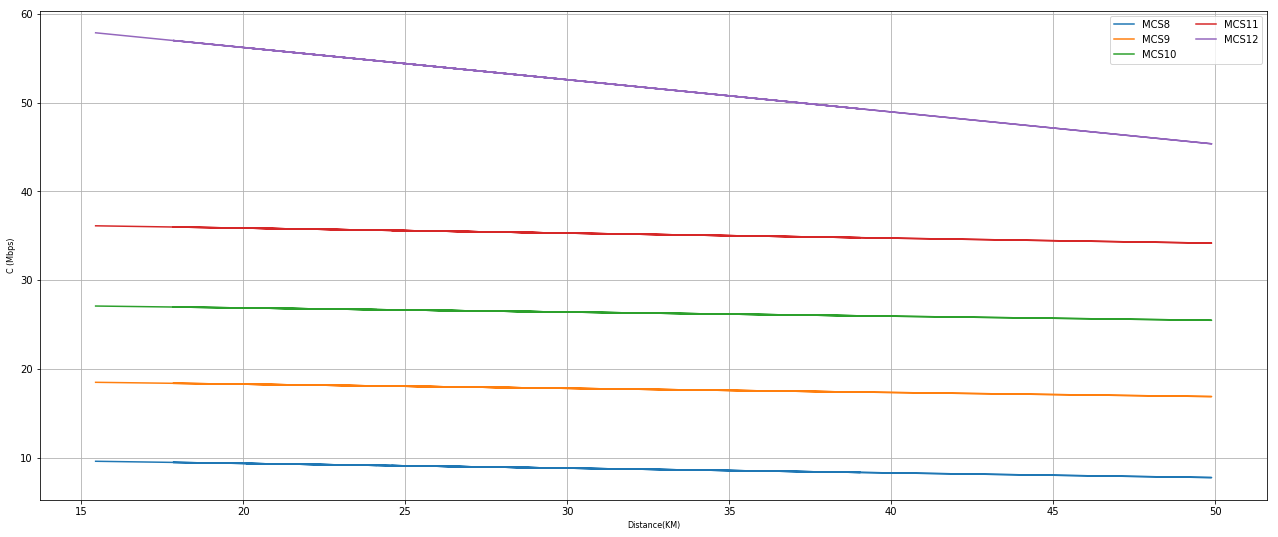
\includegraphics[width=0.7\textwidth]{img/rectas.png}
		\caption{Rectas lineales utilizando valores de 0 Km y 30 Km como coordenadas base}
		\label{rectaspendiente}
	\end{figure}
	
	\begin{figure}[H]
		\centering
		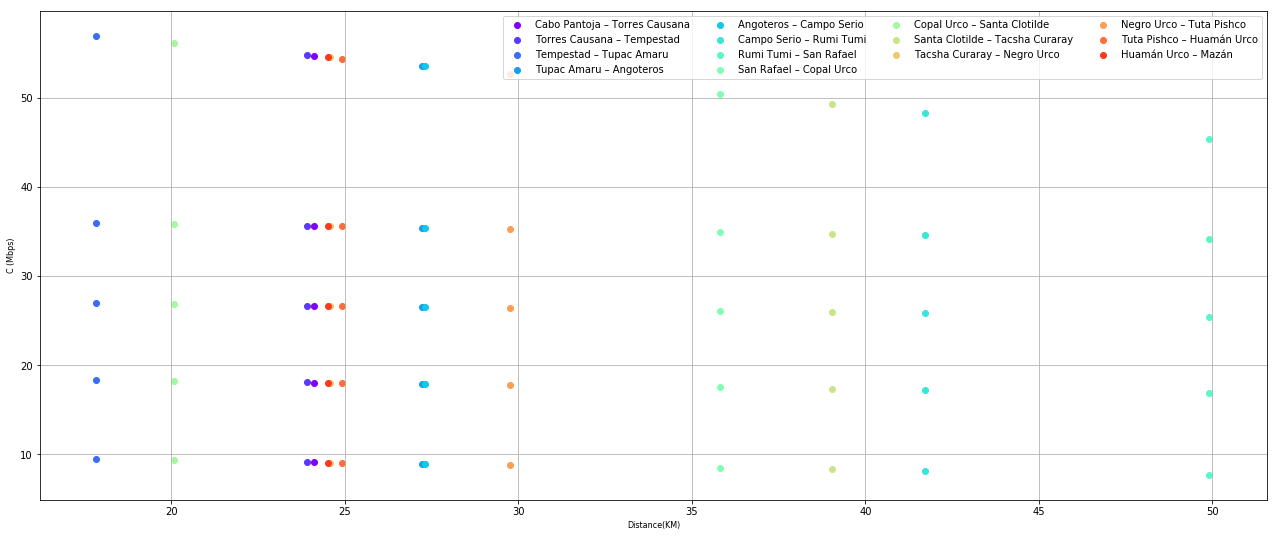
\includegraphics[width=0.7\textwidth]{img/valoresmbps.png}
		\caption{Capacidad del canal teórica respecto a la distancia para cada MCS con NV2}
		\label{valoresmbps}
	\end{figure}
	
	Los valores obtenidos y representados corresponden a las modulaciones comprendidas entre MCS8 y MCS12; no obstante, el interés de este estudio es determinar cual sería la modulación mínima utilizable de forma teórica en la red del Napo, asegurando así esa capacidad mínima definida de 44 Mbps por radioenlace. Como se ha comentado al inició del capítulo, y debido a la no disponibilidad de los valores relacionados con el \textit{throughput} para el protocolo NV2 y un ancho de banda de 40 Mhz, diseñaremos un sistema de coordenadas que relacione distancia y ancho de banda con el objetivo de aproximar los datos no conocidos respecto a 40 MHz en base a los conocidos de 20 Mhz.\\
	
	En conclusión a este análisis teórico y aproximación analítica, la Tabla \ref{table:capacidades} recoge los datos obtenidos, los cuales reflejan que para cumplir con los requesitos necesarios de la red cada radioenlace debe utilizar una modulación MCS10.   
	
\subsection{Estudio con RadioMobile}
	Una vez desarrolado el estudio teórico sobre la red, nuestro siguiente paso será realizar una representación simulada con el objetivo de obtener más información sobre la viabilidad de enlace relativa a los emplazamientos del proyecto. Para ello, utilizaremos los datos de geolocalización y distancia relacionados con los emplazamientos de la red del Napo los cuales se encuentran en las Tablas \ref{table:distancias} y \ref{table:geolocalizacion}, para introducirlos en la herramienta RadioMobile y crear así nuestra red simulada. Junto a la localización geográfica y altura de cada emplazamiento tendremos que configurar los principales parámetros de la red y de los equipos en la herramienta, esta combinación nos permitirá obtener una aproximación sobre la calidad del enlace en términos generales e individuales de la red. A continuación se detallan las características de los sistemas insertados en la herramienta para llevar a cabo la simulación:
	\begin{itemize}
		\item Potencia de transmisión: 32 dBm
		\item Sensibilidad en recepción: -96 dBm
		\item Pérdidas por cable: 1,5 dB
		\item Ganancia de antena: 30 dBm
		\item Tipo de antena: Omnidireccional
		\item Frecuencia: 5260 MHz
	\end{itemize}
	Una vez configurado los parámetros y características de los sistemas, obtenemos una representación simulada de la red tal y como se muestra en la Figura \ref{redNapo}. Dicha simulación está sujeta al modelo \textit{Longley-Rice} que utiliza la variabilidad de tiempo, posición y situación para realizar los cálculos respecto al balance de enlace.  
	\begin{figure}[H]
		\centering
		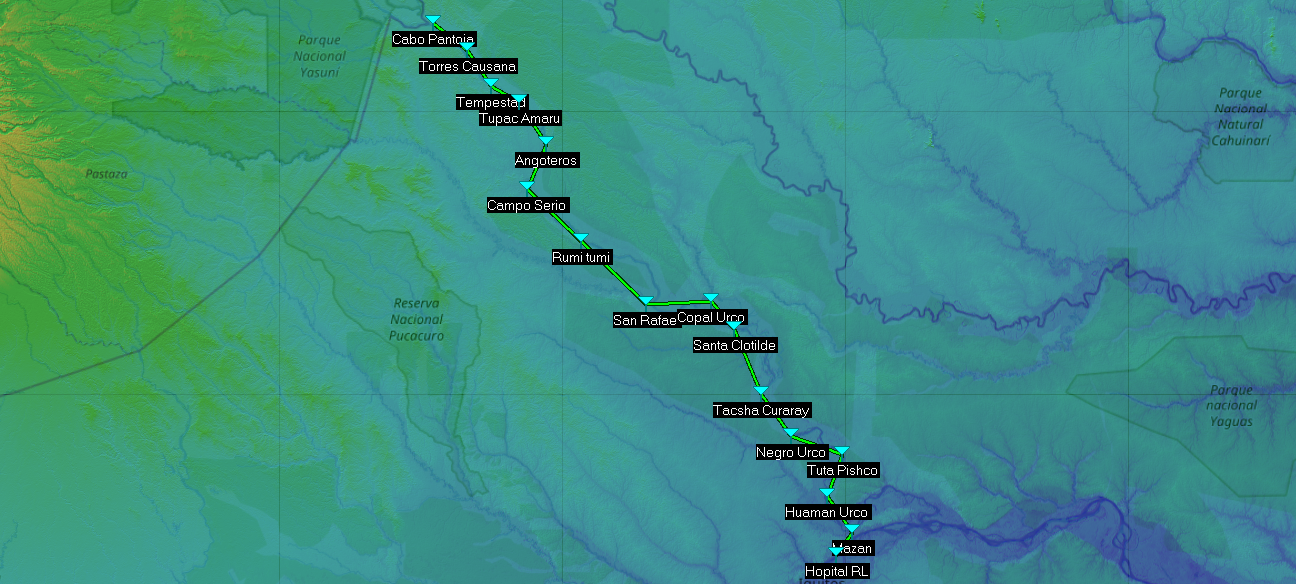
\includegraphics[width=0.7\textwidth]{img/redNapo.PNG}
		\caption{Representación de la red del Napo en RadioMobile.}
		\label{redNapo}
	\end{figure}
	La funcionalidad \textit{Radio Link} que se encuentra dentro de RadioMobile nos permite obtener una representación simulada del estado de cada radioenlace a través de la recreación del perfil geográfico y configuración de los sistemas involucrados en el enlace. Esto nos permite conocer los niveles de pérdidas, sensibilidad en recepción y margen dinámico de cada sistema de forma individual a través de la realización del balance de enlace. Dicho balance de enlace nos proporcionará información respecto a la sensibilidad y potencia en transmisión y recepción, para poder establecer la mínima tasa de transmisión soportada siempre y cuando cumpla con los requisitos de viabilidad de enlace mencionados al principio de este Trabajo Fin de Grado.\\\\
	
	Para poder obtener una tasa mínima que cumpla los requisitos de transmisión mínimos mencionados en el capítulo de introducción, debemos tener en cuenta el tipo de tecnología que estamos utilizando. En nuestro caso, las transmisiones pertenencientes a la nueva red del Napo se realizarán utilizando la tecnología \textit{Multiple Input Multiple Output}, junto al uso de NV2 como protocolo de acceso al medio. La utilización de MIMO hace que nos centremos en los valores pertenecientes a las MCS cuyos valores están comprendidos entre MCS8 y MCS15, dichas MCS a su vez están formadas desde una constelación BPSK (formada por dos símbolos) hasta una 64-QAM (formada por 64 símbolos). Para poder establecer una comparación entre la modulación adecuada por cada radioenlace tendremos que comparar la senbilidad en recepción de cada sistema obtenido mediante la simulación, con los valores típicos de sensibilidad para dichos MCS.\\
	
	Una vez expuesto el escenario y parametrización de la simulación, procedemos a realizar la misma con el objetivo de obtener la potencia recibida teórica en cada radioenlace y conocer así la viabilidad de los enlaces, los datos extraídos de esta simulación se encuentran en la Tabla \ref{table:rmEnlaceteorico}. La viabilidad de los enlaces vendrá marcado por la comparación entre le potencia teórica recibida y la sensibilidad existente para cada modulación utilizando en protocolo NV2, dichos datos se encuentran en la Tabla \ref{table:sensibilidadMCS}. A continuación, se detallan la conclusiones obtenidas del análisis simulado: 
	\begin{itemize}
		\item Existe línea de visión directa en la mayoría de casos, lo que implica asegurar la zona de Fresnel mínima para la viabilidad del enlace, en nuestro caso un sesenta por ciento.
		\item Habiendo analizado cada balance de enlace de forma individual, podemos realizar una extrapolación para el total de la red, asegurando así un margen dinámico que garantice la viabilidad del enlace. En el caso del diseño inicial dicho margen dinámico era de 20 dB, por tanto habiendo contrastado los datos obtenidos con la simulación no existe compromiso respecto a la viabilidad de enlace en cada punto de la red.
		\item En base al estudio análitico hecho, para asegurar la total funcionalidad de la red, habría que utilizar un MCS10 como mínimo para alcanzar una capacidad de enlace suficiente y necesaria.
	\end{itemize}
	
\subsection{Configuración de equipos}
Para poder recrear en laboratorio un escenario punto a punto de similares características a los de la red del Napo, utilizaremos dos equipos NetMetal 5 y dos portátiles con sistema operativo GNU/Linux. Los ordenadores portátiles actuarán de emisor y receptor en nuestra red local junto a los equipos NetMetal 5 que interconectarán dichos terminales finales entre sí, como se muestra en la Figura \ref{enlace}. Para obtener valores relacionados con los parámetros de QoS, se inyectará tráfico con la herramienta Iperf y Bandwidth test, utilizando uno de los portátiles como cliente y otro como servidor.\\\\

\begin{figure}[H]
	\centering
	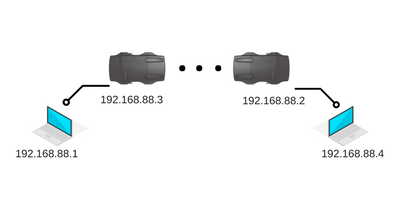
\includegraphics[width=0.7\textwidth]{img/escenario.png}
	\caption{Escenario de laboratorio punto a punto.}
	\label{enlace}
\end{figure}

Antes de comenzar a detallar cómo se ha realizado la configuración a nivel de laboratorio de los equipos, debemos apuntar que en nuestro caso las antenas utilizadas son dipolos elementales colocados en posición vertical y horizontal transmitiendo forma multimodal; en el caso del proyecto Napo cada radioenlace constará de una antena parabólica colocada en lo alto de una infraestructura metálica, cuya ganancia de transmisión está en torno a los 30 dB. \\

\section{Inyección de tráfico simulado}
Para conocer el rendimiento y prestaciones de los equipos realizaremos pruebas a nivel de red a través de la inyección de tráfico simulado. Para llevar a cabo dicha prueba, utilizaremos el software disponible para los sistemas operativos de distribución Linux Iperf y la herramienta de medida de ancho de banda proporcionada por MikroTik Bandwidth text, las cuales se detallan brevemente a continuación.\\

\subsection{Iperf}
Iperf \cite{Iperf} es una herramienta que permite realizar mediciones sobre el máximo rendimiento alcanzable respecto al ancho de banda y la calidad de un enlace red. Esto es posible mediante el análisis y recopilación de datos referentes a los protocolo de red TCP y UDP. Existe la variante Jperf, cuya única diferencia es la utilización de una interfaz gráfica en lugar de la entrada estándar de comandos.\\

La herramienta puede ser utilizada en modo cliente o en modo servidor, permitiendo realizar pruebas sobre la red hasta obtener los valores óptimos sobre la misma, tal y como se muestra en la Figura \ref{logTestIperf}.\\

Esto es gracias al ajuste y modificación de parámetros que permite la herramienta: según sea nuestro escenario y el objetivo de nuestras pruebas, podremos obtener un tipo específico de datos u otros. La elección de los parámetros de la herramienta será diferente según el protocolo de red (TCP o UDP) que utilicemos en cada caso. A continuación detallamos las posibilidades que ofrece en base a cada uno de ellos:\\

En primer lugar explicaremos los parámetros relacionados al protocolo UDP, el cual nos permite seleccionar un ancho de bando específico en nuestra comunicación y permite utilizar multidifusión si fuera necesario. Además, los datos reportados por la herramienta en este caso son los relacionados con la pérdida de paquetes, ya sea en cuantía o en porcentaje, y las medidas relacionadas con el jitter y retardo.\\

En segundo lugar, los parámetros configurables respecto a TCP están relacionados con la elección de un tamaño de ventana TCP fijo para la comunicación, otorgando datos respecto al ancho de banda medido en la comunicación y el tamaño MSS/MTU.

\begin{figure}[H]
	\centering
	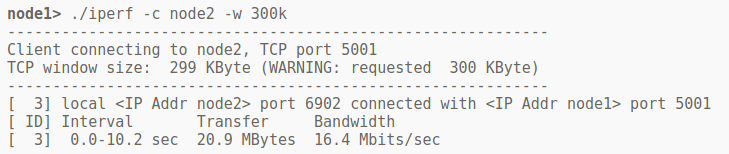
\includegraphics[width=0.7\textwidth]{img/log_iperf.png}
	\caption{Log obtenido al realizar una prueba con Iperf. Fuente: Iperf}
	\label{logTestIperf}
\end{figure}

\subsection{Bandwidth test}
\textit{Bandwidth test} es la herramienta desarrollada por el fabricante que nos permite realizar medidas entre equipos MikroTik en lo que a \textit{throughput} se refiere. Dicha herramienta está disponible tanto para la interfaz web, cómo para la consola.\\

Para llevar a cabo dicho test, debemos configurar uno de los routers que forman la red en modo servidor, y el resto en modo cliente, además la herramienta nos proporciona una serie de parámeotros configurables respecto a la red activa tales cómo: dirección, duración, tamaño de paquete, etc... \\
En función de estos parámetros el resultado de la prueba será de un modo u otro, y nos proporcionará los valores deseados respecto a el número de paquetes pérdidos, velocidades medias y totales en recepción y transmisión de la conexión activa. A continuación, en la Figura \ref{logTest} se muestra un ejemplo del log obtenido al realizar una prueba utilizando la herramienta mencionada anteriormente.

\begin{figure}[H]
	\centering
	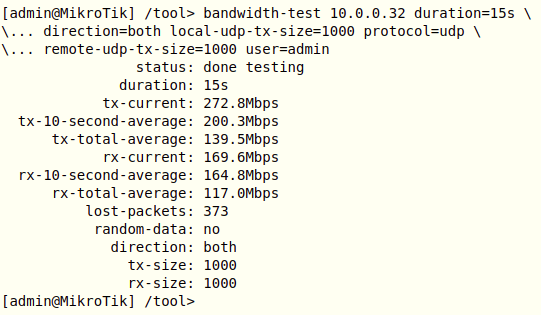
\includegraphics[width=0.7\textwidth]{img/log_test.png}
	\caption{Log obtenido al realizar una prueba sobre un enlace MikroTik activo. Fuente: Mikrotik Router and Wireless}
	\label{logTest}
\end{figure}

\section{Monitorización y gestión: Zabbix}
En esta sección se explicará la integración llevada a cabo con el escenario configurado en laboratorio y el \textit{software} de monitorización Zabbix. Así mismo, se procederá a explicar de manera más detallada el funcionamiento de la herramienta seleccionada en el marco contextual definido al inicio de este Trabajo Fin de Grado.\\

Antes de realizar la configuración del escenario formado en laboratorio, se procede a explicar cómo se va a llevar a cabo la integración de Zabbix y dicho escenario. Esto se llevará a cabo mediante el uso de plantillas XML y el protocolo SNMP, el cual nos permite intercambiar información entre los dispositivos involucrados.\\
 
El protocolo SNMP (\textit{Simple Network Management Protocol}) es un protocolo que corresponde con la capa de aplicación y facilita el intercambio de información administrativa entre los dispositivos que componen una red, ya sean \textit{routers}, \textit{switches}, etc... Este protocolo facilita a los administradores de red conocer en todo momento el estado de la red, así cómo la posibilidad de interactuar con la misma tomando acciones de prevención, resolución de problemas y estudio sobre escalabilidad.\\

Para lograr esto, SNMP accede a la MIB (\textit{Management Information Base}) de los equipos. La MIB es una colección de información referente al equipo organizada de forma jerárquica mediante un árbol, para llevar a cabo una eficiente búsqueda y consulta de los objetos que se encuentran dentro del árbol, se organizan en subconjuntos denominados organizaciones.\\\\

Cada objeto, denominado OID (\textit{Object Identifier}) contiene un valor asociado al parámetro que representa, ya sea en formato de cadena de carácteres o en formato numérico, para conseguir dicho valor se ha de realizar una búsqueda descendente del árbol que forma la MIB, ya sea bien utilizando la nomenclatura numérica que tiene cada organización seguida de un punto (1.3.6....) o bien utilizando el nombre de cada organización seguido de un punto (iso.identified....). Ambos métodos permiten recuperar el valor del parámetro deseado y utilizarlo en nuestra integración.\\

Así mismo, el funcionamiento de SNMP involucra a los siguiente agentes:

\begin{itemize}
	\item Sistema administrador: Capaz de ejecutar aplicaciones (comandos) capaces de controlar los dispositivos involucrados en la red, proporcionando métricas útiles para el administrador en cuánto a los recursos del equipo.
	\item Dispositivo administrado: Equipo que contiene el agente SNMP y forma parte de la red recogiendo información usando el protocolo SNMP.
	\item Agente SNMP: Permite realizar una administración de la forma otorgada por el equipo de manera local y jerarquizarlo en forma de árbol y en un formato compatible al intercambio de información usando dicho protocolo.
\end{itemize}

SNMP no sólo nos permite recorrer el árbol MIB y obtener información de los equipos, sino que mediante aplicaciones (comandos), es posible realizar simples operaciones sobre la estructura jerarquizada de los equipos, dichos comando se describen a continuación:

\begin{itemize}
	\item Lectura/Escritura: Permiten al administrador leer/modificar los valores de las variables almacenados dentro de los dispositivos.
	\item Notificación: Permite a los equipos reportar eventos de manera asíncrona al administrador. 
	\item Transversales: Permiten a los equipos recolectar información de los elementos cercanos en la red y conformar tablas relacionadas a la información obtenida. 
\end{itemize}

\subsection{Integración de escenario}
Una vez explicado todo lo que implica el uso de SNMP y la jerarquización de los objetos existente en los equipos y cómo es posible realizar consultas a dichos objetos, procedemos a explicar cómo se va a integrar la información procedente de los equipos con Zabbix. Una de las facilidades que nos ofrece la herramienta es que podemos crear \textit{items} tal y como se muestra en la Figura \ref{xmlTest}, aprovechando la información que nos proporcionan los OIDs en función de los parámetros que deseemos monitorizar. Para ello deberemos seguir el estándar XML, utilizando una plantilla como la mencionada antes e importarla en el sistema. De igual forma que podemos importar datos, existe la posibilidad de exportarlos, ofreciendo así versatilidad a la hora de integrar cualquier equipo en un sistema diferente. En el marco del proyecto los principales parámetros de interés son los referentes a salud de los equipos (carga CPU, temperatura, etc...) y a tráfico obtenido. 

\begin{figure}[H]
	\centering
	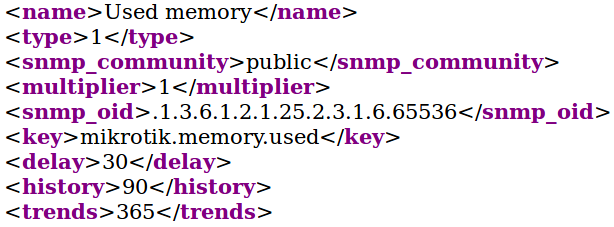
\includegraphics[width=0.7\textwidth]{img/xml_example.png}
	\caption{Ejemplo de configuración de un item sobre XML en Zabbix}
	\label{xmlTest}
\end{figure}

Una vez cargados los dispositivos involucrados en la plataforma, Zabbix ofrece varias herramientas para realizar un seguimiento sobre dichos elementos y otorgar control total sobre ellos al administrador, como por ejemplo configurando \textit{dashboards} de seguimiento, alertas sobre equipos, creación de mapas de redes, etc. A continuación se procede a detallar algunas de las aplicaciones utilizadas en este Trabajo Fin de Grado cuyo objetivo es monitorizar y obtener un control total de la red:\\

En primer lugar, nos hemos centrado en la representación gráfica del rendimiento que otorgan los equipos a nivel de red, para ello, hemos utilizado la aplicación que ofrece la propia herramienta que permite realizar gráficas a nivel de interfaz, como se muestra en la Figura \ref{zabbixMeasure}, una aplicación interesante de estas gráficas es que se puede realizar un tablero configurable conjunto, es decir, integrar dicha gráfica (o similares) de diferentes dispositivos en un único tablero, otorgando así al administrador una visión global del tráfico entrante y saliente de la red en conjunto.

\begin{figure}[H]
	\centering
	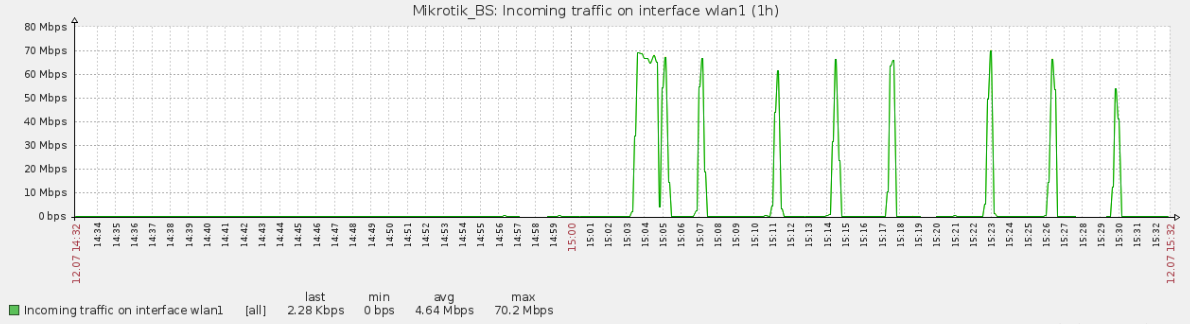
\includegraphics[width=0.7\textwidth]{img/zabbix_measure.png}
	\caption{Ejemplo de representación gráfica de tráfico mostrado en un Dashboard de Zabbix.}
	\label{zabbixMeasure}
\end{figure}

En segundo lugar, Zabbix ofrece alertas configurables en función de los \textit{items} cargados en la plantilla XML tal y como se muetra en la Figura \ref{zabbixResume}; esto quiere decir que la herramienta ofrece \textit{triggers} configurables, ya sea bien de forma predeterminada o personalizada, que permiten establecer valores umbral para los diferentes niveles de alerta que ofrece la herramienta, generando así una categorización de problemas y otorgando al administrador una versión prioritaria de la acción que ha de ser tomada. Las alertas no son configuradas únicamente si el programa se está ejecutando en primer plano, Zabbix ofrece una extensión llamada PostFix \cite{PostFix} que permite integrar y configurar alertas para que sean enviadas mediante email.\\
De igual forma, Zabbix mantiene un archivo histórico de logs el cual otorga cierta ventaja a la hora de actuar al administrador, ya sea en labores de mantemiento de la red o bien en labores predictivas. 

\begin{figure}[H]
	\centering
	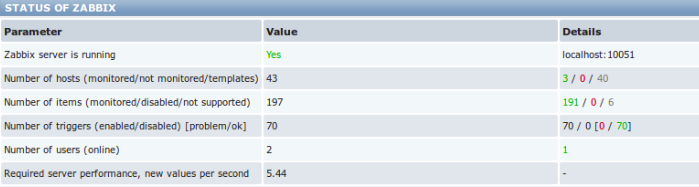
\includegraphics[width=0.7\textwidth]{img/zabbix_resume.png}
	\caption{Ejemplo del estado de la red en Zabbix}
	\label{zabbixResume}
\end{figure}

Por último, otra aplicación interesante en el marco del proyecto es la creación de mapas de red, como muestra la Figura \ref{zabbixNetwork}, la cual permite al administrador no sólo jerarquizar los equipos en función de nombres o por IPs, si no que otorga la posibilidad de subdividir una red total en subredes de forma que puedan aislarse cada una de ellas en subconjuntos, consiguiendo así un análisis más rápido y eficaz que si tuviera que realizarse de toda la red en conjunto. Aparte de esto, subdividir las redes porporciona la capacidad de asignar cada subred a un grupo de técnicos determinado evitando así que la gestión de una única subred involucre al resto de la misma.

\begin{figure}[H]
	\centering
	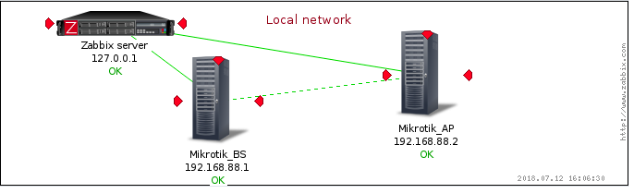
\includegraphics[width=0.7\textwidth]{img/zabbix_networks.png}
	\caption{Ejemplo de jerarquización de redes en Zabbix}
	\label{zabbixNetwork}
\end{figure}

En definitiva y reuniendo todo lo explicado a lo largo de este capítulo, Zabbix no sólo es una solución que cumple con los requisitos mínimos de monitorización de redes requeridos en el proyecto, si no que su amplia variedad de integraciones y aplicaciones.Zabbix no sólo permite una fácil integración con los dispositivos físicos mediante el uso de plantilla XML y protocolo SNMP, si no que también ofrece una solución a todo lo referido con \textit{software} de terceros. Todo esto a partir de la editabilidad de la mayor parte su funcionalidad básica para hacer que el administrador de redes tenga la mayor cantidad de información sobre los equipos, concentrada de tal forma que su actuación se inminente y precisa si esta fuera requerida.